\documentclass[a4paper,12pt,twoside,openright,titlepage]{book}

%Additional packages
\usepackage[ascii]{inputenc}
\usepackage[T1]{fontenc}
\usepackage[dutch,english]{babel}
\usepackage{syntonly}
\usepackage[official]{eurosym}
%\usepackage[graphicx]
\usepackage{graphicx}
\graphicspath{ {./images/} }
\usepackage{float}
\usepackage{xurl}
\usepackage{hyperref}
\hypersetup{colorlinks=true, linkcolor=blue, citecolor=blue, filecolor=blue, urlcolor=blue, pdftitle=, pdfauthor=, pdfsubject=, pdfkeywords=}
\usepackage{tabularx}
\usepackage{scrextend}
\addtokomafont{labelinglabel}{\sffamily}
\usepackage{listings}
\usepackage{adjustbox}

%define inch
\usepackage{mathpazo,amsmath}
\def\inch#1{#1''}

% Turn on indexing
\usepackage{imakeidx}
\makeindex[intoc]

% Support for bijlagen
\usepackage[toc,page]{appendix}

% Define colors
\usepackage{color}
\definecolor{ashgrey}{rgb}{0.7, 0.75, 0.71}

% Listing style
\lstset{
  backgroundcolor=\color{ashgrey},   % choose the background color; you must add \usepackage{color} or \usepackage{xcolor}; should come as last argument
  basicstyle=\footnotesize,        % the size of the fonts that are used for the code
  breakatwhitespace=false,         % sets if automatic breaks should only happen at whitespace
  breaklines=true,                 % sets automatic line breaking
  extendedchars=true,              % lets you use non-ASCII characters; for 8-bits encodings only, does not work with UTF-8
  frame=single,	                   % adds a frame around the code
  keepspaces=true,                 % keeps spaces in text, useful for keeping indentation of code (possibly needs columns=flexible)
  rulecolor=\color{black},         % if not set, the frame-color may be changed on line-breaks within not-black text (e.g. comments (green here))
  showspaces=false,                % show spaces everywhere adding particular underscores; it overrides 'showstringspaces'
}

% Uncomment for production
% \syntaxonly

% Style
\pagestyle{headings}

%%%%%%%%%%%%%%%%%%
% Begin document %
%%%%%%%%%%%%%%%%%%

% Define document
\author{D. Leeuw}
\title{Security: Cryptografie}
\date{\today\\v.0.1.0}

\begin{document}
\selectlanguage{dutch}

\maketitle

\copyright\ 2022 Dennis Leeuw\\

\begin{figure}[H]

\includegraphics[width=0.3\textwidth]{CC-BY-SA-NC.png}
\end{figure}

\bigskip

Dit werk is uitgegeven onder de Creative Commons BY-NC-SA Licentie en laat anderen toe het werk te kopi\"eren, distribueren, vertonen, op te voeren, en om afgeleid materiaal te maken, zolang de auteurs en uitgever worden vermeld als maker van het werk, het werk niet commercieel gebruikt wordt en afgeleide werken onder identieke voorwaarden worden verspreid.


%%%%%%%%%%%%%%%%%%%
%%% Introductie %%%
%%%%%%%%%%%%%%%%%%%

\frontmatter
\chapter{Over dit Document}
Dit boek behandelt Cryptografie.

\section*{Versienummering}
Het versienummer van elk document bestaat uit drie nummers gescheiden door een punt. Het eerste nummer is het major-versie nummer, het tweede nummer het minor-versienummer en de laatste is de nummering voor bug-fixes.\par
Om met de laatste te beginnen als er in het document slechts verbeteringen zijn aangebracht die te maken hebben met type-fouten, websites die niet meer beschikbaar zijn, of kleine foutjes in de opdrachten dan zal dit nummer opgehoogd worden. Als docent of student hoef je je boek niet te vervangen. Het is wel handig om de wijzigingen bij te houden.\par
Als er flink is geschreven aan het document dan zal het minor-nummer opgehoogd worden, dit betekent dat er bijvoorbeeld plaatjes zijn vervangen, geplaatst of weggehaald, maar ook dat paragrafen zijn herschreven, verwijderd of toegevoegd, zonder dat de daadwerkelijk context is veranderd. Een nieuw cohort wordt aangeraden om met deze nieuwe versie te beginnen, bestaande cohorten kunnen doorwerken met het boek dat ze al hebben.\par
Als het major-nummer wijzigt dan betekent dat dat de inhoud van het boek substantieel is gewijzigd om bijvoorbeeld te voldoen aan een nieuw kwalificatiedossier voor het onderwijs. Een nieuw major-nummer betekent bijna altijd voor het onderwijs dat men in het nieuwe schooljaar met deze nieuwe versie aan de slag zou moeten gaan. Voorgaande versies van het document zullen nog tot het einde een schooljaar onderhouden worden, maar daarna niet meer.

\section*{Document ontwikkeling}
Het doel is door middel van open documentatie een document aan te bieden aan zowel studenten als docenten, zonder dat hier hoge kosten aan verbonden zijn en met de gedachte dat we samen meer weten dan alleen. Door samen te werken kunnen we meer bereiken.\par
Bijdragen aan dit document worden dan ook met alle liefde ontvangen. Let u er wel op dat materiaal dat u bijdraagt onder de CC BY-NC-SA licentie vrijgegeven mag worden, dus alleen origineel materiaal of materiaal dat al vrijgegeven is onder deze licentie.

\begin{flushleft}
\begin{table}[h!]
\centering
	\begin{tabularx}{\textwidth}{ |p{0.1\linewidth}|p{0.3\linewidth}|p{0.5\linewidth}| }
\hline
	Versie &
	Auteurs &
	Wijzigingen\\
\hline
	0.7.0 &
	Dennis Leeuw &
	Uitwerking hoofdstuk Authenticiteit, plus wat updates en fixes\\
\hline
	0.3.0 &
	Dennis Leeuw &
	Toevoeging frequentie analyse, hoofdstuk over kraken is sectie geworden\\
\hline
	0.2.0 &
	Dennis Leeuw &
	Meer over Streaming en Block Ciphers, stukje over Enigma machine\\
\hline
	0.1.0 &
	Dennis Leeuw &
	Eerste release\\
\hline
\hline
\end{tabularx}
\caption{Document wijzigingen}
\label{table:1}
\end{table}
\end{flushleft}



%%%%%%%%%%%%%%%%%
%%% De inhoud %%%
%%%%%%%%%%%%%%%%%
\tableofcontents

\mainmatter

\chapter{Introductie}
\index{Cryptografie}Cryptografies betekent het schrijven (grafie) in geheim (crypto) schrift. De bedoeling is dat een tekst omgezet wordt in iets dat niet meer leesbaar is. Van klare tekst\index{Klare tekst} (leesbaar) naar een cijfertekst\index{Cijfertekst} (onleesbaar). De omzetting van klare tekst naar cijfertekst heet encryptie\index{Encryptie}. Je hebt natuurlijk niets aan een cijfertekst als je die niet weer leesbaar kan maken. Het omzetten van cijfertekst naar klare tekst heet decryptie\index{Decryptie}.

Er zijn verschillende methodes om klare tekst om te zetten naar cijfertekst. Vroeger werden de omzettingen met pen en papier gedaan de methodes die we daarvoor kennen noemen we daarom handcijfers\index{Handcijfer}, de moderne technieken gebruiken computers en wiskundige methodes en heten algoritmes\index{Algoritme}.

Binnen de wetenschap is de cryptografie een onderdeel van de wiskunde. In de cryptografie houdt men zich bezich met het beveiligen van informatie door het om te zetten in een vorm die alleen door de beoogde ontvanger(s) weer verwerkt kan worden tot bruikbare informatie. Het het kraken van bestaande encryptie-methoden behoort ook tot de cryptografie.

Om data veilig met elkaar te delen zijn er een aantal zaken belangrijk:
\begin{description}
\item[Integer] Een derde persoon kan de berichten niet veranderen
\item[Vertrouwelijk] Een derde persoon kan de berichten niet lezen (encryptie)
\item[Authentiek] Een derde persoon kan zich niet voordoen als de zender of ontvanger
\end{description}

\section{Alice en Bob}
In de security kom je vaak de karakters\index{Security Karakters} Alice\index{Alice}, Bob\index{Bob}, Eve\index{Eve} en Malory\index{Malory} tegen. Deze personen verbeelden de abstracte gedachte van data die loopt van A naar B met iemand in het Midden. Malory of Eve is de slechterick. Eve is generiek de Evil (slechte) persoon en Malory is The (Wo)Man in the Middle. Malory is afkomstig van het woord 'malice' dat kwaadaardigheid betekent. Alice en Bob betekenen niets meer dan van A naar B en hadden even goed andere namen kunnen hebben.

De karakters Alice en Bob zijn bedacht door Ron Rivest, Adi Shamir Leonard Adleman in hun artikel uit 1978 genaamd "A Method for Obtaining Digital Signatures and Public-key Cryptosystems" (\url{https://dl.acm.org/doi/10.1145/359340.359342}. Sinds het verschijnen van dit artikel zijn er vele karakters bijgekomen. Een overzicht van de verschillende karakters kan je vinden op \url{https://en.wikipedia.org/wiki/Alice_and_Bob}.


\chapter{Integriteit}
\index{Integriteit}Integriteit of in het Engels integrity\index{Integrity} gaat erover dat we kunnen nagaan of iets origineel\index{Origineel} of oorspronkelijk\index{Oorspronkelijk} is en er niet mee gerommeld is. In een paspoort zitten bijvoorbeeld heel veel grafische elementen verwerkt wat het namaken moeilijk maakt. Het zelfde geldt voor papiergeld. Er wordt bij geld bijvoorbeeld gebruik gemaakt van speciaal papier, inkt en watermerken. In je paspoort zit zelfs een chip verwerkt.

Als we niet zeker weten of een document, kunstwerk of een stuk software origineel is dan kunnen we ook niets over de waarde zeggen. Het is dus heel belangrijk dat we integriteit controleren. In de digitale techniek gebruiken we hashes om te controleren of onze digitale informatie oorsponkelijk is.

\section{Hashing}
\index{Hashing}Een van de eerste dingen die we willen weten als we een bericht naar iemand sturen is of dit correct is aangekomen en met correct bedoelen we dat er onderweg geen wijzigingen hebben plaats gevonden. Het kan natuurlijk gebeuren dat door een slechte verbinding een 1 in een 0 verandert, maar het kan ook zo zijn dat ergens onderweg iemand stiekem onze data heeft gewijzigd. Het kan bijvoorbeeld zo zijn dat als er software van Internet gedownload wordt dat aan deze software een virus hangt die tegelijk met de software ge\"installeerd wordt. Om zeker te zijn dat we de software downloaden zoals deze op de website is gezet kan een leverancier ervoor kiezen om een hash over de software te berekenen en deze uitkomst openbaar op de website te zetten. Berekenen je over de gedownloade software zelf ook de hash dan moeten deze twee gelijk zijn. Is dat het geval dan weet je zeker dat er niet met de software gerommeld is. De kunst van goede hashing software is dat er bij verschillende input nooit twee dezelfde antwoorden uit mogen komen.

Een simpele vorm van hashing zou kunnen zijn dat de hashing-software alle 1'en en alle 0'en telt en deze twee getallen achter elkaar zet. Het resultaat maakt de leverancier dan bekent. Als jij hetzelfde doet dan kan je de twee uitkomsten vergelijken. Dit is natuurlijk wel heel simpel en er is makkelijk mee te sjoemelen, toch is het principe van hashing-software hetzelfde.

MD5\index{MD5}\index{Hashing!MD5}, ofwel Message-Digest 5\index{Message-Digest 5}, is bedacht door Ronald Rivest in 1991 en kent een 128 bits hash-waarde. Dit is lange tijd een veel gebruikt hashing-algoritme geweest tot ontdekt werd dat het helemaal niet zo moeilijk was om bij verschillende input een gelijke hash-waarde te cre\"eren.

SHA\index{SHA}\index{Hashing!SHA}, ofwel Secure Hashing Algorithems\index{Secure Hashing Algorithms}, is een collectie van algoritmes. Het oorspronkelijke algoritme (nu bekend onder de naam SHA-0 of SHA) heeft maar heel kort bestaan omdat er een fout in zat. De eerste versie die wel veel gebruikt is (tot 2010) heeft een lengte van 160-bits en staat bekend als SHA-1 (of ook hier gewoon SHA). SHA-2 bestaat uit twee verschillende functies, \'e\'en met 256-bits en \'e\'en met 512-bits hash-waardes. Daarnaast is er ook nog SHA-3. Voor meer inhoudelijke informatie over SHA verwijzen we graag naar de Wikipedia-pagina \url{https://en.wikipedia.org/wiki/Secure\_Hash\_Algorithms}

Op Windows 10 is er een tool genaamd certutil.exe\index{certutil} die gebruikt kan worden om hashing-waarden te berekenen. Deze tool kan alleen vanaf de commandline gebruikt worden door de administrator.

\begin{lstlisting}[language=bash]
C:\> certutil -hashfile <PATH_TO_FILE> <HASH_ALGORITHM>
\end{lstlisting}

Het HASH\_ALGORITHM kan MD5 zijn, maar bijvoorbeeld ook SHA256.

Linux en Mac OS X hebben afzonderlijke tools voor MD5 en SHA.
\index{md5sum}\index{sha256sum}\index{sha512sum}
\begin{lstlisting}[language=bash]
$ md5sum <PATH_TO_FILE>
$ sha256sum <PATH_TO_FILE>
$ sha512sum <PATH_TO_FILE>
\end{lstlisting}

Binnen de cryptografie is het kunnen berekenen van een unique hash-waarde over een bestand of bericht essentieel.



\chapter{Vertrouwelijkheid}
\index{Vertrouwelijkheid}Vertrouwelijkheid of in het Engels Confidentiality\index{Confidentiality} is ervoor zorgen dat bepaalde informatie alleen gelezen wordt door bepaalde mensen. Dit kan bijvoorbeeld door op documenten een stempel te zetten met confidential zodat we weten dat niet iedereen die mag lezen. Je kan natuurlijk ook de documenten opbergen in een kast waarvan maar enkele personen een sleutel hebben of je bergt ze op in een kluis. In de digitale techniek gebruiken we meestal een stuk software dat informatie versleuteld zodat het onleesbaar wordt en noemen we het cryptografie.

\section{Substitutie}
\index{Substitutie}Substitutie is een ander woord (synoniem) voor vervanging. In de cyptografie betekent dat dat je een letter of cijfer vervangt door iets anders. Dat anders kan een andere letter zijn of een cijfer inplaats van een letter, maar ook bijvoorbeeld een symbool. Hoewel nooit bedoeld als geheimschrift is de Morse code ook een vorm van substitutie. Elke letter is vervangen door een korter en/of langer signaal om een boodschap over te brengen.

Meer informatie over de Morse code: \url{https://en.wikipedia.org/wiki/Morse_code}

\subsection{Caesarcijfer}
\index{Caesarcijfer}\index{Caesarrotatie}\index{Substitutie!Rotatie}E\'en van de oudste vorm van substitutie cryptografie die we nog kennen is de Caesarcijfer (Caesarrotatie), gebruikt door Julius Caesar (100 v. Chr - 44 v. Chr.) om te voorkomen dat zijn bevelen in handen vielen van vijanden als zijn boodschappers onderweg overvallen en vermoord werden. De substitutie cryptografie die Caesar gebruikte bestond uit het verschuiven van de letters in het alfabet. Een verschuiving van 1 betekende dat alle letters A een B worden, alle letters B een C, etc. Een verschuiving van 4 kan er dan zo uit zien:

%% \begin{tabularx}{\textwidth}{ | c | c | c | c | c | c | c | c | c | c | c | c | c | c | c | c | c | c | c | c | c | c | c | c | c | c | }
%% \hline
%%  a & b & c & d & e & f & g & h & i & j & k & l & m & n & o & p & q & r & s & t & u & v & w & x & y & z \\ 
%% \hline
%%  w & x & y & z & a & b & c & d & e & f & g & h & i & j & k & l & m & n & o & p & q & r & s & t & u & v \\
%% \hline
%% \end{tabularx}

\begin{tabular}{ | c | c | c | c | c | c | c | c | c | c | c | c | c | c | c | c | c | c | c | }
\hline
 a & b & c & d & e & f & g & h & i & j & k & l & m & n & o & p & q & r & s \\ 
\hline
 w & x & y & z & a & b & c & d & e & f & g & h & i & j & k & l & m & n & o \\
\hline
\end{tabular}

\begin{tabular}{ | c | c | c | c | c | c | c | }
\hline
 t & u & v & w & x & y & z \\ 
\hline
 p & q & r & s & t & u & v \\
\hline
\end{tabular}

Als we in ons bericht in klaretekst de letter opzoeken in de bovenste regel en dan de letter uit de regel eronder noteren op een nieuw papiertje dan kunnen we de geencrypte tekst versturen zonder dat iemand meteen kan lezen wat er staat. Een voorbeeld:

\begin{verbatim}
Beste Bob, we gebruiken vandaag de Caesarrotatie, Groet Alice.
xaopa xkx, sa caxnqegaj rwjzwwc za ywaownnkfwpea, cnkap wheya.
\end{verbatim}

Een andere naam voor de vorm van encryptie is ROT\index{ROT} van rotatie. De bovenstaande encryptie heet dan ROT4 omdat de letters 4 posities zijn opgeschoven. Een bijzondere vorm is de ROT13\index{ROT13}:

\begin{tabular}{ | c | c | c | c | c | c | c | c | c | c | c | c | c | }
	\hline
 a & b & c & d & e & f & g & h & i & j & k & l & m \\
	\hline
 n & o & p & q & r & s & t & u & v & w & x & y & z \\
	\hline
\end{tabular}

Het nadeel van de Caesarrotatie is dat er maar 25 verschillende mogelijkheden zijn die simpel \'e\'en voor \'e\'en te testen zijn. In Caesar zijn tijd waarin veel mensen niet lezen konden was dit minder een probleem. Het wat de elite die kon lezen en dan moesten ze ook nog instaat zijn om te begrijpen dat het om cryptografie ging om het bericht te ontsleutelen.

Meer informatie: \url{https://nl.wikipedia.org/wiki/Caesarcijfer}


\subsection{codebook}
\index{Codebook}\index{Substitutie!Codeboek}In de codeboek versleuteling gaat het om de omzetting van hele stukken tekst door een andere. Er worden dan zinsdelen omgezet door gebruik te maken van dezelfde omzettingstabel. Stel dat een generaal een bericht over wil brengen over hoe troepen zich moeten verplaatsen. Bijvoorbeeld: \textquote{Infanterie devisie 304 naar het noorden.} Als we afspreken dat \textquote{infanterie divisie 304} aangeduid wordt als \textquote{de olifant} en \textquote{het noorden} is \textquote{de oever}, dan zou de tekst kunnen worden \textquote{De olifant naar de oever}. Voor de vijand zegt dit niets als ze niet over dezelfde codebook beschikken. De hoeveelheid combinaties is theoretisch eindeloos, maar het is nog steeds zo dat de substitutie vast is, dus altijd zal \textquote{infanterie divisie 304} vertaald worden met \textquote{de olifant}, dus als je maar genoeg berichten onderschept en voldoende troepen bewegingen waarneemt dan zal je uiteindelijk ontdekken welk zinsdeel wat betekent.


\subsection{Rozenkruizers}
\index{Rozenkruisers}\index{Substitutie!Symbolen}Een andere vorm van substitutie is het vervangen van letters en cijfers door symbolen. E\'en van de bekende vormen is die van de Rozenkruisers. de oudste variant is afkomstig uit 1533 en is beschreven in de "occulta philosophia" van Agrippa\index{Agrippa} von Nettesheim. Agrippa was een geleerd man uit Duitsland, geboren in Keulen in 1486 en gestorven in Grenoble in 1535. Zijn code kan beschreven worden zoals weergegeven in figuur \ref{fig:rosenkruisen}.

\begin{figure}[h!]
	\centering
	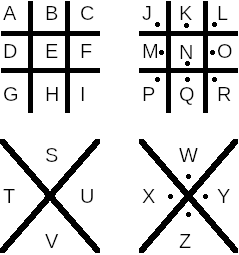
\includegraphics[width=0.4\linewidth]{Rozenkruisen.png}
	\caption{Rosenkruiserscode}
	\label{fig:rosenkruisen}
\end{figure}

Het deel waar de letter in staat is het symbool waardoor de letter vervangen wordt. Een a wordt dus een 

\includegraphics[height=\fontcharht\font`\B]{Rozenkruisen_A.png}
en een W wordt dan 

\includegraphics[height=\fontcharht\font`\B]{Rozenkruisen_W.png}
. Zo kunnen we ook zinnen maken, probeer maar eens uit te vinden wat hier staat:


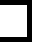
\includegraphics[height=\fontcharht\font`\B]{Rozenkruisen_d.png} 
\includegraphics[height=\fontcharht\font`\B]{Rozenkruisen_i.png} 
\includegraphics[height=\fontcharht\font`\B]{Rozenkruisen_t.png} \, 
\includegraphics[height=\fontcharht\font`\B]{Rozenkruisen_i.png} 
\includegraphics[height=\fontcharht\font`\B]{Rozenkruisen_s.png} \, 
\includegraphics[height=\fontcharht\font`\B]{Rozenkruisen_e.png} 
\includegraphics[height=\fontcharht\font`\B]{Rozenkruisen_e.png} 
\includegraphics[height=\fontcharht\font`\B]{Rozenkruisen_n.png} \, 
\includegraphics[height=\fontcharht\font`\B]{Rozenkruisen_z.png} 
\includegraphics[height=\fontcharht\font`\B]{Rozenkruisen_i.png} 
\includegraphics[height=\fontcharht\font`\B]{Rozenkruisen_n.png}.

Hoewel minder makkelijk leesbaar is de decodering ook hier weer simpel omdat voor elke letter het symbool uniek is, dus er zijn maar 26 verschillende symbolen. Met voldoende tekst is deze versleuteling eenvoudig te kraken.

\section{Kolomtranspositie}
\subsection{Matrix}
De meest eenvoudige manier om een bericht te versleutelen is het gebruik van een matrix. In de tabel \ref{tab:matrix} hebben we de zin 'Deze zin wordt versleuteld' uitgeschreven in een matrix van 5x5.
\begin{table}[h]
\centering
\begin{tabular}{|c|c|c|c|c|}
\hline
	D &
	e &
	z &
	e &
	z \\
\hline
	i &
	n &
	w &
	o &
	r \\
\hline
	d &
	t &
	v &
	e &
	r \\
\hline
	s &
	l &
	e &
	u &
	t \\
\hline
	e &
	l &
	d &
	0 &
	0 \\
\hline
\end{tabular}
\caption{Bericht in een matrix}
\label{tab:matrix}
\end{table}
Door de tekst op te schrijven van boven naar beneden krijgen we de cijfertekst: didse entll zwved eoeu0 zrrt0. Degene die deze geheime boodschap onderschept moet het formaat van de matrix weten om uit te vinden wat het bericht is. In het voorbeeld hebben we het geencrypte bericht uitgeschreven in blokken van 5, dat is natuurlijk niet zo handig en ook de twee 0'en verraden al veel, maar als we de 0'en vervangen door willekeurige letters en er 1 lange reeks letters van maken dan wordt het al weer een stuk moeilijker om de matrix te raden.

\subsection{Matrix met passphrase}
Als we dezelfde zin versleutelen met een passphrase\index{Passphrase} wordt de encodering nog een stukje complexer. Een passphrase is hetzelfde als een wachtwoord of een key\index{key} (sleutel\index{sleutel}), maar hoeft deze niet perse een woord te zijn, maar kan het ook een hele zin zijn. In de matrix \ref{tab:matrix_passphrase} gebruiken we 'bosje' als passphrase. We schrijven eerst de passphrase in de tabel, deze bepaalt daardoor hoe breed onze tabel wordt. Onder de passphrase zetten we getallen en die verwijzen welke letter het eerst in het alfabet voorkomt. In ons voorbeeld is de 'b' letter die het meest vooraan in het alfabet staat, dus die krijgt waarde \textbf{1} de 'e' is de erop volgende letter en die krijgt dus waarde \textbf{2} en zo voort. De dikgedrukte nummering bepaalt nu de volgorde waarin we de kolom uitlezen.

\begin{table}[h]
\centering
\begin{tabular}{|c|c|c|c|c|}
\hline
	b &
	o &
	s &
	j &
	e \\
\hline
	\textbf{1} &
	\textbf{4} &
	\textbf{5} &
	\textbf{3} &
	\textbf{2} \\

\hline
\hline
	d &
	e &
	z &
	e &
	z \\
\hline
	i &
	n &
	w &
	o &
	r \\
\hline
	d &
	t &
	v &
	e &
	r \\
\hline
	s &
	l &
	e &
	u &
	t \\
\hline
	e &
	l &
	d &
	f &
	g \\
\hline
\end{tabular}
\caption{Bericht in een matrix}
\label{tab:matrix_passphrase}
\end{table}
De cijfertekst wordt dan: didse zrrtg eoeuf entll zwved. De passphrase bepaalt op deze manier hoe de kolommen uitgelezen worden.


\section{Het kraken van de cijfertekst}
\subsection{Frequentie-analyse}
Veel van de handmatige cijfers zijn te kraken door gebruik te maken frequentie analyse\index{Frequentie analyse}. Frequentie analyse is een techniek waarbij er gekeken wordt welke letters er in een taal in welke aantallen voorkomen. Door ervan uit te gaan dat elke encrypte tekst een gemiddelde verdeling heeft kunnen op basis van het voorkomen van bepaalde letters met een bepaalde frequentie de oorspronkelijke letters ingevuld worden. In figuur \ref{fig:NEfreq} staat de frequentie analyse van de Nederlandse taal. Hierbij is duidelijk dat de e de meest voorkomende letter is. Vinden we nu een encrypte tekst waarin p de meest voorkomende letter is dan kunnen we de p vervangen door de e. Als we zo alle letters af gaan dan kunnen we vele letters plaatsen en het bericht weer lezen.

\begin{figure}[h]
	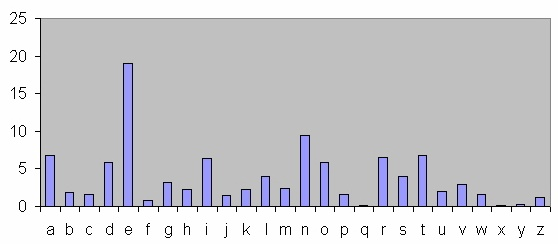
\includegraphics[width=\textwidth]{NEfreq.jpg}
	\caption{Frequentie Analyse van de Nederlandse taal (\href{https://commons.wikimedia.org/wiki/File:NEfreq.jpg}{CC SA}: Natastia at Dutch Wikipedia)}
	\label{fig:NEfreq}
\end{figure}

Met computers en digitale woordenboeken kunnen dit soort analyses heel snel gedaan worden. Het is natuurlijk wel belangrijk om te weten in wat voor taal het oorspronkelijke bericht was opgesteld.

\subsection{Enigma machine}
De Engima\index{Enigma} machine is populair geworden door zijn gebruikt door de Nazi's en het feit dat de geallieerden de code konden breken en de berichten mee konden lezen. Toch is de techniek al ouder dan de tweede wereldoorlog.

De Enigma gebruikt een rotor mechanisme om de 26 letter van het alfabet door elkaar te gooien. Bij het intoetsten van een letter op het toetsenbord lichte een letter op op het scherm boven het toetsenbord. De oplichtende letter was de encrypte variant. Dus voor elke toets aanslag moest de oplichtende letter opgeschreven worden, wat vaak door een tweede persoon gedaan werd. Als de encrypte tekst werd ingetoetst dan verscheen op het scherm de bijbehorende gedecodeerde letter, zo kon het oorspronkelijke bericht weer zichtbaar gemaakt worden. Het rotor mechanisme veranderde de verbindingen tussen de toetsten en de lampjes na elke toetsaanslag, dus elke letter werd unique gecodeerd.

Om te zorgen dat de machine niet elke keer alles op dezelfde manier codeert moet hij (dagelijks) worden voorzien van een nieuwe key, die beide partijen moeten kennen, dus een vorm van de one-time-pad. De lijsten met codes moeten dus van te voren bij de verzendende en ontvangende partij bekend zijn en beide partijen moeten op hetzelde moment van key wijzigen.

Het oorspronkelijke ontwerp werd al in 1932 gekraakt door een Poolse wiskundige: Marian Rejewski. Ook de verbeteringen die de Duitsers aanbrachten gedurende de oorlog werden steeds opnieuw gebroken, zodat de Polen en later de geallieerden met Poolse nagemaakte Enigma's de meeste berichten van de Duisters konden blijven volgen.

\section{Onkraakbare cijfertekst}
\subsection{One-time pad}
De onbreekbare code\index{Onbreekbare code} bestaat en die heet: One-time pad\index{One-time pad} (OTP\index{OTP}). De one-time pad maakt gebruik van modulo rekenen (zie Appendix \ref{chap:modulo}).

Er zijn een aantal eisen waaraan de versleuteling met een one-time pad moet voldoen:
\begin{enumerate}
\item \label{nl:secret} De sleutel moet volledig geheim gehouden worden en mag alleen bekend zijn aan de versleutelaar en aan degene die het bericht moet ontcijferen
\item \label{nl:reuse} De sleutel mag niet in zijn geheel of gedeeltelijk herbruikt worden (vandaar one-time)
\item \label{nl:length} De sleutel moet net zo lang of langer zijn dan het bericht dat versleuteld wordt
\item \label{nl:random} De sleutel moet bestaan uit volledig willekeurige (random) waarden. Er mag dus geen algoritme worden gebruikt, maar er moet zoiets gebruikt worden als een hardware random number generator
\end{enumerate}

In tabel \ref{tab:onetimepad} staan 2 rijen volledig willekeurige cijfers (eis \ref{nl:random}). Ze zijn opgedeeld in blokken van 10 cijfers en er zijn 5 blokken per rij. Dat betekent dat we 100 willekeurige cijfers hebben. Als we een bericht schrijven in alleen hoofdletters en de letters omzetten via de ASCII tabel \url{https://en.wikipedia.org/wiki/ASCII} dan hebben we voor de letters A tot Z de decimale getallen 65 tot 90 nodig. We gebruiken dus 2 cijfers per letter. Met een maximale sleutellengte van 100 cijfers kunnen we dus maximaal een bericht van 50 characters versturen om te blijven voldoen aan eis \ref{nl:length}.

\begin{table}[h!]
\begin{tabular}{ | c | }
\hline
	Serial: 5837424 \\
\hline
	7867562615 8641646198 7616531254 5327516761 2563621687 \\
	5674816856 9887216521 9563201567 3618568716 5768716568 \\
\hline
\end{tabular}
\caption{One-time pad}
\label{tab:onetimepad}
\end{table}

Als een spion een bericht wil versturen dan stelt hij eerst zijn bericht op van maximaal 50 tekens (zie regel 1 uit tabel \ref{tab:otp:encrypt}), per letter zet hij de waarde van de ASCII tabel er onder (zie regel 2 uit tabel \ref{tab:otp:encrypt}) en dan net zoveel cijfers van de one-time pad als nodig is om even veel cijfers te hebben als er voor het bericht nodig zijn (zie regel 3 van tabel \ref{tab:otp:encrypt}). Tot slot komt er nog wat reken werk. We tellen het eerste cijfer van het eerste karacter op bij het eerste cijfer van de sleutel en daarna het tweede cijfer van het eerste karakter op bij het tweede cijfer van de sleutel, daar het eerste cijfer van het tweede karakter bij het derde cijfer van de sleutel, etc. (zie regel 4 van tabel \ref{tab:otp:encrypt}) en tot slot bereken we van de twee verkregen cijfers bij elk karakter de modulo 10 (mod10) en zetten we de uitkomst weer achter elkaar zodat we per karakter weer een getal hebben van 2 cijfers (zie regel 5 van tabel \ref{tab:otp:encrypt}).

\begin{table}[h!]
\setlength\tabcolsep{1.5pt}
\centering
\begin{tabular}{ | c || c | c | c | c | c | c | c | c | c | c | c | c | }
\hline
	1 & O    & P    & H    & A    & L     & E    & N    & O    & P    & J    & F    & K  \\
	2 & 81   & 80   & 72   & 65   & 76    & 69   & 78   & 81   & 80   & 74   & 70   & 75 \\
	3 & 78   & 67   & 56   & 26   & 15    & 86   & 41   & 64   & 61   & 98   & 76   & 16 \\
	4 & 15 9 & 14 7 & 12 8 & 8 11 & 8 11  & 14 15& 11 9 & 14 5 & 14 1 & 16 12& 14 6 & 8 11 \\
	5 & 59   & 47   & 28   & 81   & 81    & 45   & 19   & 45   & 41   & 62   & 46   & 81 \\
\hline
\end{tabular}
\caption{OTP: Encrypt}
\label{tab:otp:encrypt}
\end{table}

De spion moet hierna het serienummer van het bericht opschrijven plus de gemaakt te cijferreeks: 5837424594728818145194541624681 en deze code is volledig onbreekbaar. Alleen degene met een papiertje met hetzelfde serienummer en dus dezelfde sleutel kan dit bericht decoderen.

Het decoderen verloopt door het omgekeerde proces te doorlopen. We verwijderen eerst het serienummer van de reeks en zetten de overgebleven losse cijfers in een rij (regel 1 van tabel \ref{tab:otp:decrypt}. Plaats daar onder de cijfers van de sleutel (regel 2 van tabel \ref{tab:otp:decrypt}. Trek het sleutelgetal van het cijfergetal af, is de uitkomst negatief tel dan 10 op bij het cijfergetal (het getal uit het bericht) en trek nogmaals het sleutel getal ervan af (regel 3 van tabel \ref{tab:otp:decrypt}. En tot slot zoek je de gevonden waarden op in de ASCII tabel zodat op regel 4 het oorspronkelijke bericht weer verschijnt.

\begin{table}[h!]
\centering
\begin{tabular}{ | c || c | c | c | c | c | c | c | c | c | c | c | c | }
\hline
	1 & 5 9 & 4 7 & 2 8 & 8 1 & 8 1  & 4 5 & 1 9 & 4 5 & 4 1 & 6 2 & 4 6 & 8 1 \\
	2 & 7 8 & 6 7 & 5 6 & 2 6 & 1 5  & 8 6 & 4 1 & 6 4 & 6 1 & 9 8 & 7 6 & 1 6 \\
	3 & 8 1 & 8 0 & 7 2 & 6 5 & 7 6  & 6 9 & 7 8 & 8 1 & 8 0 & 7 4 & 7 0 & 7 5 \\
	4 &  O  &  P  &  H  &  A  &  L   &  E  &  N  &  O  &  P  &  J  &  F  &  K \\
\hline
\end{tabular}
\caption{OTP: Decrypt}
\label{tab:otp:decrypt}
\end{table}


\chapter{Digitale cryptografie}
\section{Symmetrisch}
Als een bericht encrypt is zullen we deze ook weer willen decrypten. Als we voor het encrypten en voor het decrypten dezelfde sleutel of methode gebruiken dan noemen we dat symmetrische encryptie. Symmetrische encryptie en decryptie is snel, maar kent het nadeel dat de sleutel voor beide partijen bekent moet zijn. De vraag bij symmetrische encryptie is altijd hoe je ervoor zorgt dat alle partijen die een bericht moeten kunnen lezen de sleutel krijgen zonder dat deze zomaar over een onveilig medium (zoals het Internet) verstuurd wordt.

\subsection{Streaming cipher}
In een streaming cipher\index{Streaming cipher} wordt de klare tekst gecombineerd met een keystream van random data waarbij de klare tekst en de random data gecombineerd worden, bit voor bit. Een streaming cipher wordt gebruikt als we niet weten hoeveel data er komen gaat.

De keystream moet net zo lang of langer zijn als het te encrypten bericht en mag natuurlijk maar \'e\'en keer gebruikt worden. Door deze eisen is een werkelijke digitale implementatie van de one-time pad zeer lastig en wordt deze slechts zelden gebruikt. Het probleem is vooral het veilig delen van de key.

De meeste streaming ciphers maken gebruik van een keystream die gegenereerd wordt op basis van een key (bijvoorbeel 128-bits), hierdoor is de keystream niet volledig random en spreken we van een pseudorandom keystream. Hierdoor is het bewijs dat de one-time pad onbreekbaar is niet geldig voor deze streaming ciphers, maar wordt deze wel vaak gebruikt in praktische toepassingen.

Een streaming cipher maakt gebruik van een XOR. RC4 is \'e\'en van de meest bekende streaming ciphers. Een overzicht van andere stream ciphers is te vinden op \url{https://en.wikipedia.org/wiki/Stream_cipher}


RC4\index{RC4} is een van de meest bekende streaming ciphers die gebruikt wordt. RC4 wordt tegenwoordig niet meer als veilig gezien. RC4 staat voor Rivest Cipher versie 4\index{Rivest Cipher 4}.

RC4 wordt gebruikt door SSL\index{SSL} (Secure Socket Layer\index{Secure Socket Layer}) en WEP\index{WEP} (Wired Equivalent Privacy\index{Wired Equivalent Privacy})


\subsection{Block cipher}
Een Block Cipher\index{Block Cipher} wordt gebruikt als we weten hoeveel data we moeten versturen. Een Block Cipher gebruikt een omzetting die vergelijkbaar is met een transpositie matrix. De omzetting geschiedt per block (bijvoorbeeld 128 bits) en gebruikt voor het encrypten een symmetrische sleutel. De key is in moderne algoritmes evenlang of langer dan het te encrypten datablock.

Block ciphers gebruiken pseudorandom keys.

De bekendste Block Ciphers zijn AES (Advanced Encryption Standard), DES (Data Encryption Standard), Triple DES en Blowfish.


DES\index{DES} is eigenlijk een aangepaste versie van Lucifer\index{Lucifer} een van de eerste Block Ciphers ontwikkeld door IBM. De Amerikaanse overheid koos het als standaard (Data Enryption Standard\index{Data Encryption Standard}) in 1976. DES heeft een block grootte van 64 bits en een sleutel lengte van 56 bits. De kleine sleutel lengte is de zwakte van het systeem en DES wordt dan ook niet meer als veilig gezien. Sinds 1998 is aangetoond dat DES gebroken kan worden.


De opvolger van DES is AES\index{AES} (Advanced Encryption Standard\index{Advanced Encryption Standard}). De wedstrijd voor een nieuwe standaard werd gewonnen door Joan Daemen en Vincent Rijmen, twee Belgische cryptografie wetenschappers, die wat zij de Rijndael cipher noemden instuurden. AES heeft een block grootte van 128-bits en gebruikt sleutels van 128, 192 of 256-bits. AES gebruikt een 4x4 bytes matrix.


\subsection{Symmetrisch versleuteling en het Internet}
Voor het sturen van data over Internet via bijvoorbeeld een website is een uitdaging voor symmetrische encryptie. Om echt onbreekbaar te zijn moeten we aan de volgende eisen voldoen:
\begin{itemize}
\item Volledige random key
\item Key net zo lang als het bericht
\item Zender en ontvanger gebruiken dezelfde sleutel voor encryptie en decryptie
\item Sleutel mag maar 1x gebruikt worden
\end{itemize}

Een beetje pagina op Internet bevat, html-pagina, met CSS-document, 1 of meerdere javascript documenten, plaatjes, etc. Voor elk van deze stukken data hebben we dus een sleutel nodig die net zo lang is als het stuk data (video), die volledig random moet zijn en maar 1x gebruikt mag worden. Daarnaast moeten de webserver en de browser allebei deze sleutel hebben. Dus op de een of andere manier moet die sleutel over het Internet getransporteerd worden, op een veilige manier.

Het volledig random genereren van data (sleutel) kan met een Hardware Random Number Generator\index{Hardware Random Number Generator}\index{HRNG} (HRNG). De meeste Random Number Generators\index{Random Number Generator}\index{RNG} gebruiken een sleutel om semi-random waarden te cre\"eeren en worden daarom Pseudo-Random Number Generators(PRNG)\index{Pseudo-Random Number Generator}\index{PRNG} genoemed. Met een PRNG voldoen we dus al niet meer aan de eis van echte onbreekbaarheid, toch wordt dit het meest gebruikt omdat het wel praktisch en relatief goedkoop toepasbaar blijft.

De lengte stelt ons bij video's al snel voor een probleem. We moeten een sleutel maken die net zo lang is als de video en dus net zoveel ruimte in beslag neemt als de video.

Ook het feit dat de zender en de ontvanger over dezelfde sleutel moeten beschikken kan een probleem opleveren, hoe zorgen we ervoor dat de ontvanger dezelfde sleutel krijgt als welke de verzender gebruikt heeft terwijl we alleen het onveilige Internet hebben om de sleutel over te versturen?

\section{Asymmetrisch}
Als we een bericht willen decrypten dat encrypt is en we gebruiken voor het encrypten een andere sleutel dan voor het decrypten dan noemen we de vorm asymmetrisch. Asymmetrische encryptie vraagt om bijzondere wiskundige algoritmes waardoor deze over het algemeen trager is dan symmetrische encryptie.

\subsection{Public en Private Key}
Asymmetrische encryptie is encryptie met public\index{Public key} en private keys\index{Private key}. De private key (sleutel) wordt zoals de naam al zegt geheim (priv\'e) gehouden, de public key wordt openbaar gemaakt. Iemand die iets geheims te versturen heeft gebruikt de openbare private key om het bericht te versleutelen. Alleen degene met de private key kan het bericht nu ontsleutelen (decrypten). Voor twee wegverkeer is het dus noodzakelijk dat beide partijen een private key hebben en dat de andere partij de publieke key kent.

Encrypt je iets met de private key, dan kan iedereen die de publieke sleutel heeft het bericht decrypten. Dat heeft dus niets met beveiliging te maken. Het is wel een handige feature waar we later op terug komen.

Met een public/private key combinatie kan op een veilige manier een symmetrische key worden uitgewisseld.

Er zijn verschillende technieken op Internet die gebruik maken van public/private cryptografie. HTTPs (TLS), S/MIME, PGP (GPG) zijn wel de voornaamste technieken die we bijna dagelijks gebruiken om onze data veilig over het Internet te sturen. Er zijn verschillende algritmes die gebruikt kunnen worden, de veiligheid van de verschillende algoritmes hangt erg van van de toepassing waarvoor ze gebruikt worden. Het is ook van belang welke andere systemen ermee moeten kunnen werken. Voor HTTPs is het natuurlijk van belang dat zoveel mogelijk systemen het gebruikte algoritme ondersteunen, dus hier zal een andere keuze gemaakt worden dan bijvoorbeeld het encrypten van documenten van het Pentagon waar security vele malen belangrijker is en de uitwisseling juist geen rol speelt.

\begin{description}
\item[RSA] Rivest-Shamir-Adleman. De veiligheid van dit algoritme hangt van de key size af. 3072 of 4096 bits zijn nog veilig. Kleiner dan 2048 is onveilig. RSA bestaat al sinds 1977, dus er zijn veel implementaties voor veel systemen, dus dit algortime wordt door heel veel systemen ondersteund.
\item[DSA] Digital Signature Algorithm. Is onveilig en zou niet meer gebruikt moeten worden, vanaf OpenSSH 7.0 per default gedisabled.
\item[ECDSA] Elliptic Curves DSA. Redelijk veilig, een beetje afhankelijk van de random number generator die gebruikt wordt. Minimaal 256 bits key size.
\item[ed25519] Op dit moment (2021) de meest veilige optie, maar ook de nieuwste dus niet overal al aanwezig.
\end{description}

Voor het maken van een public/private key pair zijn dus een aantal zaken van belang:
\begin{itemize}
	\item Key algoritm
	\item Key size
	\item Passphrase - Er kan op de private key aan passphrase gezet worden, maar dit hoeft niet.
\end{itemize}

Het maken van een public/private key paar is simpel. Op Linux en Mac OS X systemen kan je ssh-keygen gebruiken, op Windows PuTTYgen, of ook met ssh-keygen (command line) als je OpenSSH voor Windows hebt ge\"installeerd.

\section{Key Exchange}
Encryptie en decryptie met symmetrische algoritmes is vele malen sneller dan met asymmetrische methodes. We willen in de digitale cryptografie dan ook ze snel mogelijk gebruik maken van een symmetrische sleutel, de vraag daarbij is hoe we zorgen dat een sleutel veilig wordt uitgewisseld tussen twee systemen. Deze sleutel uitwisseling noemen we in het Engels de key exchange\index{Key exchange}\index{Sleutel uitwisseling}.

Er zijn een aantal methodes om symmetrische sleutels met elkaar uit te wisselen:
\begin{description}
\item[Key Encapsulation Mechanism (KEM)] Door gebruik te maken van asymmetrische encryptie om een veilige verbinding op te zetten en dan daarna een symmetrische sleutel uit te wisselen.
\item[Key Exchange (KEX)] En algoritme om keys te berekenen zonder dat de te gebruiken symmetrische sleutel over de lijn gaat, zoals Diffie-Hellman (DH).
\item[Out-of-Band] De symmetrische key delen via bijvoorbeeld een USB-stick, papier, of een andere methode.
\end{description}


\subsection{Diffie-Hellman}
In 1975 waren er twee wiskundigen, Whitfield Diffie\index{Diffie, Whitfield} en Martin Hellman\index{Hellman, Martin}, die een oplossing bedachten voor het probleem van het uitwisselen van symmetrische sleutels (symmetric keys). Ze kwam met een elegante wiskundige oplossing die het versturen van de sleutel over het Internet overbodig maakt. De sleutel wordt berekend door gebruik te maken van modulo rekenen (zie appendix \ref{chap:modulo}) en priemgetallen (getallen die alleen door 1 en zichzelf deelbaar zijn). De techniek die gebruikt wordt is naar hun vernoemd: Diffie-Hellman\index{Diffie-Hellman}, afgekort DH\index{DH}.

Tabel \ref{tab:dh} beschrijft welke acties Alice en Bob moeten nemen om tot een gezamenlijke sleutel te komen. Terwijl Alice en Bob werken om tot een gezamenlijke sleutel te komen is Eve aanwezig die al het verkeerd tussen Alice en Bob afluisterd, want ook zij wil graag die geheime sleutel hebben.

\begin{table}[h]
\centering
	\begin{tabularx}{\textwidth}{ | c | X | m{1cm} | X | m{1cm} | X | }
	\hline
	Actie & Alice & & Eve & & Bob \\
	\hline
	& \multicolumn{5}{p{0.86\textwidth}|}{Alice en Bob spreken twee getallen af: p en q. De getallen zijn niet geheim en mogen over het Internet verstuurd worden. De eisen zijn dat beide getallen priemgetallen moeten zijn en dat q kleiner moet zijn dan p. Eve heeft nu p en q} \\
	\hline
	1 & $p=11$ & \centering-> & p, q & \centering<- & $q=7$ \\
	\hline
	& \multicolumn{5}{p{0.86\textwidth}|}{Alice en Bob verzinnen ieder een eigen getal dat ze geheim houden en niet met elkaar delen.} \\
	\hline
	2 & $a=3$ & & & & $b=6$ \\
	\hline
	& \multicolumn{5}{p{0.86\textwidth}|}{Alice en Bob gebruiken modulo rekenen om A en B te berekenen.} \\
	\hline
	3 & $A=q^a\%p$ & & & & $B=q^b\%p$ \\
	  & $A=7^3\%11$ & & & & $B=7^6\%11$ \\
	  & $A=2$ & & & & $B=4$ \\
	\hline
	& \multicolumn{5}{p{0.86\textwidth}|}{Alice en Bob sturen hun berekende getallen, A en B, naar elkaar. Eve heeft nu ook A en B} \\
	\hline
	4 & $A=2$ & \centering-> & A, B & \centering<- & $B=4$ \\
	\hline
	& \multicolumn{5}{p{0.86\textwidth}|}{Alice en Bob gebruiken modulo rekenen om S te berekenen} \\
	\hline
	5 & $S=B^a\%p$  & & & & $S=A^b\%p$ \\
	  & $S=4^3\%11$ & & & & $S=2^6\%11$ \\
	  & $S=9$       & & & & $S=9$ \\
	\hline
	& \multicolumn{5}{p{0.86\textwidth}|}{Eve heeft tijdens de afspraken van Alice en Bob meegeluisterd op de lijn en heeft nu de getallen p, q en A, B verzameld. Ze mist echter a of b om ook S te kunnen berekenen. Op deze manier hebben Alice en Bob via een rekenkundige weg een gezamenlijke sleutel S afgesproken zonder dat deze over het Internet gegaan is.} \\
	\hline
\end{tabularx}
\caption{DH uitleg}
\label{tab:dh}
\end{table}

Omdat de sleutel berekend wordt via een algortime (modulo rekenen) voldoet deze niet aan de eisen van een onbreekbare code, namelijk dat de sleutel volledig random moet zijn. In de praktijk is de techniek echter zo goed, als we maar voldoende grote priemgetallen nemen, dat we van een veilige verbinding kunnen spreken.

Diffie-Hellman houdt geen rekening met de identiteit van de zender en/of ontvanger, dus een man-in-the-middle attack is nog steeds mogelijk. Het gebruik van public en private keys lost dit probleem op.

\section{Hoe veilig is een algoritme?}
De veiligheid van een algoritme wordt beschreven in het aantal pogingen dat er nodig is om de sleutel te breken. Met het steeds sneller worden van compters kunnen er steeds meer pogingen gedaan worden in dezelfde tijd. De eis van het NIST is op dit moment dat een algoritme beter moet zijn dan 128-bits, $2^128$ pogingen voordat het gebroken wordt. De veronderstelling is dat we daarmee tot 2030 vooruit kunnen. Voor RSA betekent dat een minimum van 3072 bits key size.


Om te bepalen welke cipher suites je wel en niet wil toestaan is er een site die voor je bijhoudt welke suites geschikt zijn en welke je absoluut niet meer moet gebruiken omdat ze te makkelijk te kraken zijn. Deze site is te vinden op \url{https://ciphersuite.info/cs/?singlepage=true&security=secure}. Door de optie security=secure mee te geven zie je alleen de suites die een kwalificatie secure of hoger hebben.


\chapter{Authenticiteit}
Als we communiceren over het Internet hoe weten we dan dat bijvoorbeeld de website van de bank daadwerkelijk de website van de bank is en niet een website opgezet door een boef? Of hoe weten we zeker dat de e-mail die we gekregen hebben daadwerkelijk verzonden is door degene die in het afzenderveld staat? Al deze vragen hebben te maken met authenticiteit\index{Authenticiteit} of Authenticity\index{Authenticity} in het Engels. In het niet digitale leven zou je iemand om zijn paspoort of rijbewijs kunnen vragen zodat de persoon kan aantonen wie die is. In de digitale wereld gebruiken servers certificaten om aan te tonen dat zij echt de server van de bank zijn. Een certificaat is dus te vergelijken met een digitaal paspoort.

\section{PKI}
PKI\index{PKI} staat voor Public Key Infrastructure\index{Public Key Infrastructure} en is het totaal van maatregelen en instanties die nodig zijn om publieke sleutels te beheren. PKI is bedoelt om gebruikers en apparaten te authenticeren in een digitale wereld, vergelijkbaar met het paspoort in de gewone wereld. Het gaat daarbij om vertrouwen, vertrouwen in de echtheid van bijvoorbeeld een website die je bezoekt, de echtheid van een document, of het vertrouwen dat een gebruiker die gebruik wil maken van een systeem ook werkelijk die gebruiker is.

Vertrouwen tussen digitale entiteiten wordt bepaald door het vertrouwen dat we hebben in de public key van een entiteit. De private key moet altijd geheim blijven, maar de publieke sleutel mogen we met iedereen delen. De vraag bij de verkregen publieke sleutel is altijd of dit de sleutel is van de machine of persoon waarmee ik contact wil hebben of dat er ergens een man-in-the-middle zit die mij een valse sleutel heeft gegeven en dus stiekem met ons meeleest.

Er zijn verschillende oplossing om dit vertrouwen te bewerkstelligen:
\begin{description}
\item[CA] Certificate Authority
\item[WoT] Web of Trust
\end{description}

\subsection{Certificate Authority}
Voordat jij vertrouwd wordt om op Schiphol in een vliegtuig te stappen moet je eerst je paspoort laten zien. In je paspoort zit een foto en een beschrijving van een aantal lichamelijke kenmerken waardoor de douane beambte kan controleren dat jij en je paspoort bij elkaar horen. Het feit dat de douane beambte het paspoort vertrouwd heeft te maken met een aantal zaken. Allereerst zal hij of zij het controleren op echtheidskenmerken, zoals watermerken etc. Als dat echt blijkt te zijn, dan is de onderliggende aanname dat het document is uitgeven door de overheid en dat de overheid voor uitgifte een aantal controles heeft gedaan zodat de overheid weet dat het paspoort ook echt bij jou hoort. Het is dus de overheid die ervoor zorgt dat jij alleen jouw paspoort hebt en ook alleen jij het paspoort hebt. Tevens is het paspoort maar beperkt geldig.

Al deze dingen koment we ook tegen bij het digitale paspoort, het certificaat, dat door de Certificate Authority\index{Certificate Authority} (CA\index{CA}) wordt uitgegeven. Als je een certificaat nodig hebt, dan zul je dat moeten aanvragen. Om dit te kunnen doen moet je eerst een public en private key paar genereren. Op basis van de public key maak je een Certificate Signing Request\index{Certificate Signing request} CSR\index{CSR}. In dit verzoek tot het tekenen van het certificaat neem je een aantal zaken op zoals bijvoorbeeld waar het certificaat voor bedoeld is. Als het voor een webserver is dan neem je de domeinnaam op in het CSR, de geldigheidsduur en de eigenaar van de website. Dit verzoek stuur je op naar een CA. De CA controleert de gegevens. Dus die kijkt na of jij echt de eigenaar bent van het domein en of jij echt bent wie je bent. Als alles klopt dan krijg je van de CA een certificaat met de gegevens uit de CSR, maar nu getekend met de handtekening van de CA. De CA ondertekend het document met zijn private key. Hiermee heb je het digitale paspoort waarmee je kan aantonen dat jouw server de echte server is die bij je domeinnaam hoort.



Het paspoort waarmee een webserver aantoont dat die echt de enige echte is heet een certificaat\index{Certificaat} en net als een paspoort moet een certificaat door een instantie uitgegeven worden. Paspoorten worden uitgegeven door de gemeente (overheid) en certificaten door Certificate Authorities\index{Certificate Authority} (CA\index{CA}). Een certificaat bevat:
\begin{itemize}
\item De public key van de server
\item De domeinnaam waarvoor het certificaat geldig is
\item De geldigheidsduur
\item De handtekening (signature) van de CA
\end{itemize}

Een voorbeeld van een signature is te zien in figuur \ref{img:cert:letsencrypt}.

\begin{figure}[h]
\centering
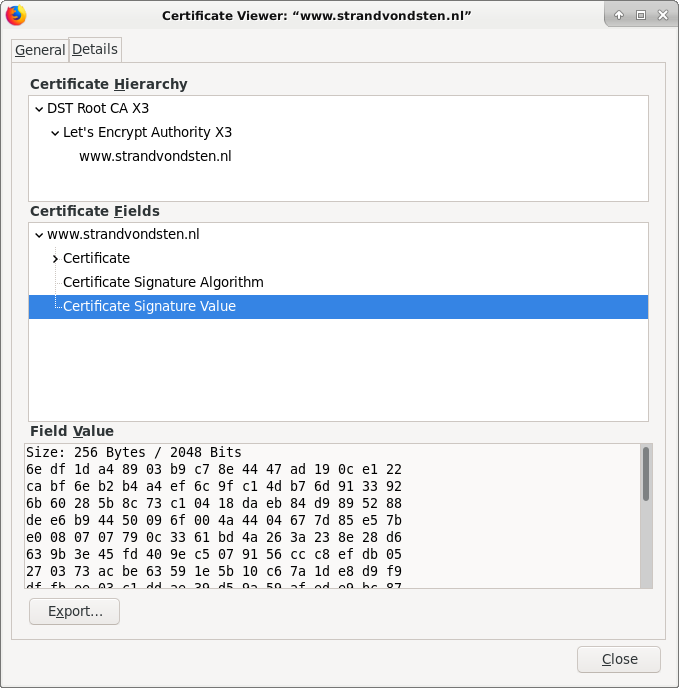
\includegraphics[width=0.8\textwidth]{Certificaat_LetsEncrypt.png}
\caption{Let's Encrypt certificaat}
\label{img:cert:letsencrypt}
\end{figure}

Een webserver heeft dus zijn eigen private key en een certificaat ge\"installeerd staan. Het stuurt zijn certificaat op aan een gebruiker (browser), die controleert het certificaat en als het goed bevonden wordt gebruikt het de public key uit het certificaat om een encrypt bericht aan de server te sturen die dat bericht can decrypten met zijn private key.

\subsection{Web of Trust}
Het Web of Trust\index{Web of Trust} (WoT\index{WoT}) is ooit bedacht door Phil Zimmermann in 1992 toen hij bezig was met PGP\index{PGP}, Pretty Good Privacy\index{Pretty Good Privacy}. Dit is gebaseerd op onderling vertrouwen zoals in een vriendenkring. Als Bob Alice vertrouwt en Alice vertrouwt Carlos dan zou Bob Carlos ook kunnen vertrouwen. Er is dus geen centrale partij die bepaalt of een certificaat of een publieke sleutel te vertrouwen is en er is ook niet \'e\'en web of trust, net zomin als er \'e\'en vriendenkring is. Er kunnen verschillende vriendenkringen wereldwijd zijn met hun eigen collectie van publieke sleutels die ze vertrouwen.

PGP is ooit ontworpen om e-mail veilig te maken. De gedachte voor de Web of Trust is dat als je public keys met je vrienden uitwisseld je een database kan opbouwen in je e-mail client en als jij aangeeft dat je deze public keys daadwerkelijk van je vrienden hebt gekregen dan ben jij degene die kan zeggen dat ze echt zijn. Als anderen dat ook doen, dan kan je daarna fysiek of electronisch de verzamelde sleutels met elkaar uitwisselen. Daarbij zou het handig zijn als je een gradatie van vertrouwen zou kunnen aangeven. Bob vertrouwt Alice, dus die sleutels zijn volledig te vertrouwen, maar Bob kent Carlos niet, dus het vertrouwen in de sleutels van Carlos zouden een iets lagere vertrouwens waarde kunnen krijgen dan die van Alice.

Het web of trust zoals dat ge\"implementeerd is in PGP en GPG\index{GPG} (GNU Privacy Guard\index{GNU Privacy Guard}, de open source implementatie van de OpenPGP\index{OpenPGP} standaard, heeft de mogelijkheid om ook gebruik te maken van een CA. Binnen een organistatie kan een eigen CA opgezet worden die de certificaten die de public keys bevatten kan certificeren. Op deze manier kan door het vertrouwen van \'e\'en certificaat alle certificaten binnen een web of trust vertrouwd worden.

\section{Signing}
Zoals al eerder aangegeven kan je met een private key berichten encrypten en deze de wereld in sturen, allen met de public key zijn deze berichten te decrypten, maar omdat iedereen bij de publiek kan is dit geen beveiliging, het is wel een vorm van authenticatie, Het is een vorm die we signing\index{signing} noemen. Een ieder die de public key heeft kan het bericht decrypten, maar weet op dat moment wel 100\% center dat het bericht encrypt is door de degene met de private key. Het is dus een bewijs dat alleen degene die de private key heeft het bericht heeft kunnen versturen. Hiermee kan dit gebruikt worden om bijvoorbeeld contracten te ondertekenen.


\begin{appendices}
	\chapter{Modulo rekenen}\label{chap:modulo}
Voor het rekenwerk binnen de crypografie hebben we soms modulo rekenen\index{Modulo rekenen} nodig, ofwel klok rekenen\index{Klok rekenen}. Modulo rekenen wordt wel klok rekenen genoemd omdat dat de meest bekende vorm is die iedereen bijna dagelijks uitvoert. Als iemand tegen je zegt we spreken om 13:00 uur af dan weet iedereen dat die persoon 1 uur 's middags bedoelt. We hebben in gedachte even snel 12 van 13 afgetrokken en hielden 1 over. Modulo rekenen is dus een rekenvorm waarbij we de rest waarde berekenen op basis van een grondgetal. Dat grondgetal bij het klokrekenen is 12. We zouden wiskundig kunnen schrijven 13 mod 12 = 1. Onze klok gaat niet verder dan 24 uur en dus ik klok rekenen een heel beperkte versie van modulo rekenen.

Als we een klok zouden nemen die iets verder doorloopt dan zouden we kunnen zeggen we spreken af om 25:00 uur. 25 mod 12 is weer 1, want we kunnen 2x12 aftrekken van 25 en dan blijven we met een rest 1 achter wat dus weer 1 uur is, alleen nu wel midden in de nacht. Ook de basis kunnen we natuurlijk veranderen: 25 mod 5 is 0, want 5x5 is 25 en 25-25 = 0. We hebben dan dus geen rest getal. Of 38 mod 3 is 2, want 12x3 is 36 en 38-36 = 2.

In programmeertalen en op rekenmachines wordt modulo rekenen vaak weergegeven met een \%. We schrijven dan 25\%12=1, of 25\%5=0.

	\chapter{De XOR}\label{chap:xor}
Een veel gebruikte functie uit de boolean algebra in de cryptografie is de XOR. Het principe van de XOR is gebaseerd op het optellen van bits waarbij alleen het laatste digit wordt gebruikt:
\begin{lstlisting}{language=bash}
0 + 0 = 0
1 + 0 = 1
0 + 1 = 1
1 + 1 = 0
\end{lstlisting}

Daarmee komt de waarheidstabel van de XOR op de tabel zoals weergegeven in \ref{tab:xor}

\begin{table}[h]
\centering
\begin{tabular}{ | c | c | c| }
	\hline
	Input & Input & Output \\
	Input A & Input B & A XOR B \\
	\hline
	0 & 0 & 0 \\
	\hline
	0 & 1 & 1 \\
	\hline
	1 & 0 & 1 \\
	\hline
	1 & 1 & 0 \\
	\hline
\end{tabular}
\caption{XOR}
\label{tab:xor}
\end{table}

Computers kunnen via een XOR heel snel een stroom met bits encrypten. De manier waarop dat gebeurt is weergegeven in tabel \ref{tab:xor:encrypt}.

\begin{table}[h]
\centering
	\begin{tabular}{ |c|c|c|c|c|c|c|c|c| }
		\hline
		Klare tekst stream & 0 & 1 & 1 & 0 & 0 & 1 & 0 & 1 \\
		\hline
		Sleutel    & 1 & 0 & 1 & 1 & 0 & 1 & 1 & 0 \\
		\hline
		\hline
		Cijfertekst& 1 & 1 & 0 & 1 & 0 & 0 & 1 & 1 \\
		\hline
	\end{tabular}
	\caption{XOR Encrypt}
	\label{tab:xor:encrypt}
\end{table}

Het leuke van de XOR functie is dat je ook weer een XOR gebruikt voor de decryptie en dat zie er dan uit zoals in tabel \ref{tab:xor:decrypt}
\begin{table}[h]
\centering
	\begin{tabular}{ |c|c|c|c|c|c|c|c|c| }
		\hline
		Cijfertekst stream & 1 & 1 & 0 & 1 & 0 & 0 & 1 & 1 \\
		\hline
		Sleutel            & 1 & 0 & 1 & 1 & 0 & 1 & 1 & 0 \\
		\hline
		\hline
		Klare tekst        & 0 & 1 & 1 & 0 & 0 & 1 & 0 & 1 \\
		\hline
	\end{tabular}
	\caption{XOR decrypt}
	\label{tab:xor:decrypt}
\end{table}

\end{appendices}

%%%%%%%%%%%%%%%%%%%%%
%%% Index and End %%%
%%%%%%%%%%%%%%%%%%%%%
%\backmatter
\printindex
\end{document}

%%% Last line %%%
